\chapter{Ist-Analyse ( 5 \%)}
\label{chap:ist-analyse}

Dieses Kapitel dient der Beschreibung existierender System.
Es soll ihre Eigenschaften und Probleme aufzeigen.
Diese werden zuerst Theoretisch betrachtet und
dann an Systemen in der Praxis demonstriert.

% dieses kap dient .. und damit soll .. aufbau

\section{Eigenschaften der existierenden Systeme}

\subsection{Struktur}
\label{sec:ist-analyse:struktur}

Wie in der folgenden Grafik leicht zu erkennen,
sind traditionellen CI-Systeme Client-Server Systeme.

\begin{figure}[ht]
  \centering
  \label{fig:ist-aufbau-tradition}
  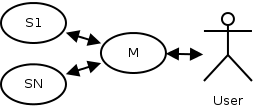
\includegraphics[height=1in]{imageinput/ist-aufbau-tradition.png}
  \caption{Logischer Aufbau eines CI System}
\end{figure}

Der sogenannte Master ist der Server und verwaltet alle Daten.
Die Slaves sind die Clients und verrichten die eigentliche Arbeit.
Sie sammeln Daten und liefern diese einschließlich der Resultate beim Master ab.

Benutzer interagieren Ausschließlich mit dem Master.

\subsection{Datensammlung}
Wie bereits in \Cref{sec:base:ci} erwähnt,
führt ein CI-System nicht nur Aufträge aus,
sondern sammelt auch Daten für die spätere Weiterverarbeitung.

Die Datensammlung lässt sich dabei grob in 2 Bereiche einteilen.
Zum einen die Laufzeitdaten und zum anderen die Artefakte.

Laufzeitdaten fallen bereits w\"ahrend der Ausf\"uhrung an,
und beinhalten in der Regel zumindest die Textuellen Ausgaben
der ausgef\"uhrten Programme.
Weitere M\"oglichkeiten k\"onnen Resultate von Tests, Echtzeit Mitschnitte und Aufführungsstatistiken sein.
Laufzeitdaten werden dem Benutzer in der Regel Zeitnah zur Verfügung gestellt.

Artefakte hingegen sind Dateien,
welche erst nach Abschluss eines Schrittes zur verf\"ugung stehen.
Zu ihnen geh\"oren neben den traditionellen ausf\"uhrbaren Dateien
auch lauff\"ahige Archive des Gesammtprogrammes oder Testergebnisse in Formaten wie z.b. JunitXML oder TAP.

%XXX: cite tap, junitxml

Diese werden zum Master geschickt, dort aufbewahrt und sp\"ater genutzt.

In der Regel werden ausf\"uhrbare Artefakte zum Download angeboten,
w\"ahrend Testergebnisse nur dargestellt werden.


\section{Probleme existierender Systeme}

Diese Sektion gibt einen \"Uberblick \"uber die Problemarten existierender Ststeme

\subsection{Datenzugriff}

Beim Datenzugriff sind die existierenden Systeme besonders Problematisch.
Es gibt Grundsätzlich keinerlei Standardschnittstellen.
Die meisten Systeme verwenden noch nicht einmal eine Datenbank.
Jene welche doch eine verwenden wird, machen sie nicht zugänglich.

Die Datenhaltung dieser Systeme kann somit grob als geordnete Ablage klassifiziert werden.
Weiterführende Abfragen sind nicht möglich.

\subsection{Erweiterbarkeit}

Die Erweiterbarkeit eines CI-Systemes wird von 2 Hauptpunkten dominiert.
Dies ist die Integration in die Benutzeroberfl\"ache
und zum anderen die Möglichkeiten mit den Daten interagieren
und auf neue Weise zu kombinieren.

Die erweiterbaren Systeme stellen normalerweise zumindest eine Schnittstelle
für die graphische Oberfläche zur Verfügung.
Damit ist zumindest das problemlose Anpassen der Benutzeroberfläche gegeben.


Für eigene Analysewerkzeuge kann es jedoch oft notwendig werden,
eine eigene Datenbank, welche vom CI-System getrennt ist zu verwenden.
Einige Anbieter von CI-Werkzeugen wünschen dies sogar explizit.
%XXX:


\subsection{Komponentenabhängigkeit}

Wie bereits in Kapitel~\ref{sec:ist-analyse:struktur} erw\"ahnt,
sind CI-Systeme in der Regel traditionelle Netzwerksysteme die nach dem Client/Server Prinzip operieren.
Dabei sind die Rollen strikt als Master und Slave eingeteilt
und das Management wird zentral im Master vorgenommen.
Slaves haben dabei keinerlei Autonomie und folgen strikt den Anweisungen des Master.

Dadurch nimmt das System zwar keinen Schaden wenn ein Slave ausfällt,
der Ausfall des Master ist jedoch fatal und kann nicht abgefangen werden.
Dies stellt einen ``Single Point of Failure'' dar.


\section{Beispiele aus der Praxis}

Um Probleme in der Praxis aufzuzeigen,
soll eine Auswahl an Werkzeugen getroffen werden.
Anschließend sollen ihre Eigenschaften und Probleme
näher untersucht werden.


\subsection{Auswahl}

Um die Analyse von Praxisbeispielen zu ermöglichen,
sollen Systeme mit gewissen Rahmenbedingungen ausgew\"ahlt werden.
Wichtigstes Kriterium ist dabei, dass sie \textbf{open-source} Software sind,
oder zumindest öffentlich verfügbar sind.
Sie sollten \textbf{verbreitet} sein, damit ein Überblick
über praxisrelevante Probleme geschaffen.
Außerdem sollten sie \textit{kostenlos} sein. %,
%XXX> LOL
%\textit{um den finanziellen Ruin eines hilflosen Studenten zu verhindern}.

Ausgewählt wurden die Systeme
\begin{itemize}
  \item Jenkins/Hudson
  \item Buildbot
  \item TravisCI
\end{itemize}

Sie alle sind kostenlose Werkzeuge und Quell-offen.
Außerdem Decken sie sehr verschiedene Use-Cases ab.

\subsection{Jenkins/Hudson}

Jenkins und Hudson sind aus der Java Welt  stammende CI-Systeme.
Sie bieten alle Grundfunktionen, um grundlegendes CI umzusetzen
und unterst\"utzen auch erweiterte Funktionen,
wie Matrix-Build und nach-gelagerte Builds.

Sie stellen ein einfach zu bedienendes Nutzerinterface zur Verfügung,
Konfiguration findet jedoch nur im Rahmen dieses Interfaces statt.

Erweiterte Parametrisierung ist nicht m\"oglich.
Auch Entwicklungszweige sind dem System unbekannt.
M\"ochte man mehr als einen Entwicklungszweig dem Testprozess unterziehen,
so m\"ussen weitere Jobs angelegt werden.

Zugriff auf die Daten kann nur mittels der internen API oder
einer nicht dokumentierten REST API genommen werden.

Damit war es nicht m\"oglich in annehmbarer Zeit festzustellen,
in wie weit sich die bereits vorgestellten UseCases umsetzen lassen.
Das System verwendet augenscheinlich kein DBMS.
Datenabfragen und Aggregationen m\"ussen
somit von Hand ausformuliert werden.

Das Konzept der Build-Artefakte wird unterst\"utzt und
aktiv f\"ur Funktionen wie nachgelagerte Builds verwendet.

Es gibt einige einfach gestrickte Plugins mit dem Zweck, Testresultate anzuzeigen.
Jedoch wird auf weitergehende Analysen dieser Resultate g\"anzlich verzichtet,
mehr als eine Historie gibt es nicht.


\subsection{Buildbot}


BuildBot \cite{buildbot:website} positioniert sich als eine Art Meta-Build-Server.
Er bietet keine normale Benutzerschnittstelle zur Konfiguration,
sondern wird mittels Komposition von Metadaten und Komponenten konfiguriert.

Die Konfiguration des Servers stellt dabei ein Pythons-Script,
welches die gewünschten Jobs zusammenstellt und den Server konfiguriert.
Matrix-Builds werden nicht unterst\"utzt,
k\"onnen aber in Teilen durch die Verwendung von Schleifen im Script simuliert werden.
Es ist möglich Builds Jobs mit minimalen Parametern in Form von Strings zu \"ubergeben,
dabei kann man auch den Entwicklungszweig mit angeben.

Builbot unterst\"utzt das Sammeln von Daten in sog. Logdateien,
diese sind intern und extern leicht auffindbar.
Es gibt sogar schon Werkzeuge, welche dies zum erweiterten Vergleichen von Testresultaten nutzen nutzen.

%XXX referenzen
%XXX: C
Einige wurden dabei besonders genau betrachtet.
Das erste ist der PYPY Buildbot \cite{pypy:overview} , welcher eine hilfreiche Gesamtübersicht der Testergebnisse und ihrer Fehler gibt
der letzten 4 Builds darstellt.
Das zweite ist das Script namens \verb|compare\_last\_builds.py|
aus dem PYPY Projekt \cite{pypy:diffscript} ,
welches die Unterschiede in den Testresultaten zwischen 2 Builds hervorhebt.
Sie werden sp\"ater als Ideenlieferant dienen.

Bedauerlich ist, das die Entwickler von BuildBot es nicht als Aufgabe ihres Systems sehen,
sich mit Testergebnissen zu befassen.
Sie empfehlen Integration externer Komponenten \cite{buildbot:irc}.

\subsection{TravisCI}


%XXX refs
TravisCI \cite{travisci:website} ist wesentlich anders positioniert, als die beiden vorhergehenden Systeme.
Es setzt Zusammenarbeit in den Vordergrund und der Open-Source Community werden gehostete Server
kostenfrei zur Verf\"ugung gestellt.
Diese behandeln die Integration von Projekten,
welche auf der beliebten Code-Hosting Site GitHub verwaltet werden.

% ref yaml
Die Konfiguration ist dabei zweigeteilt,
eine Datei im YAML Format \cite{yaml:website} legt dabei Build-Achsen und Schritte fest.
Diese Datei befindet sich in Versionskontrolle beim Projekt
(was die Konfiguration sehr flexibel gestaltet).

Ist ein Projekt erst einmal im System registriert,
so wird es regelm\"assig bei Änderungen integriert.

Besonders hilfreich ist dabei, das TravisCI auch den Fall behandelt,
wenn ein anderer Benutzer der Code-Hosting Seite Github \"Anderungen anmeldet
\cite{github:pullreq} (sog. Pull-request).
Die testet es und f\"ught anschliessend das Resultat der \"Anderungsanmeldung hinzu.

Was leider nichts daran \"andert, das TravisCI keine externe API zur Verfügung stellt.
Es ist ein geschlossenes System, außerdem hat es kein Konzept f\"ur Datensammlung/Artefakte
und auch Testresultate werden nicht betrachtet.
Es ist nicht portabel und scheinbar f\"ur den Betrieb nur
auf den zur Verfügung gestellten Servern vorgesehen.


\section{Zusammenfassung}

Dieses Kapitel hat die Probleme der CI-Systeme n\"aher gezeigt.
Wir haben gesehen, dass Datenzugriff und Erweiterungen f\"ur Analyse,
schwer oder gar nicht zu erreichen sind.
Außerdem sind die Systeme nach einigen Fehlerklassen nicht direkt wiederherstellbar.
Im folgenden Verlauf der Arbeit soll der Grundstein f\"ur ein CI-System gelegt werden,
welches Datenzugriff und Datenanalyse vereinfacht.
Zus\"atzlich soll es grundsätzliche Fehlertoleranz aufweisen.


